
\chapter{Renderings of simuated cells} % (fold)
\label{cha:renderings_of_simuated_cells}

\newcommand{\cellrenderingwidth}{8cm}
\newcommand{\cellrenderingheight}{8cm}

All renderings rendered using VMD\cite{humphrey_vmd_1996} and tachyon\cite{stone_em_1998} (internal). Colorscale is BGR (from blue at the beginning of the trajectory over green in the middle to red at the end of the trajectory).

\begin{figure}[H]
\centering
  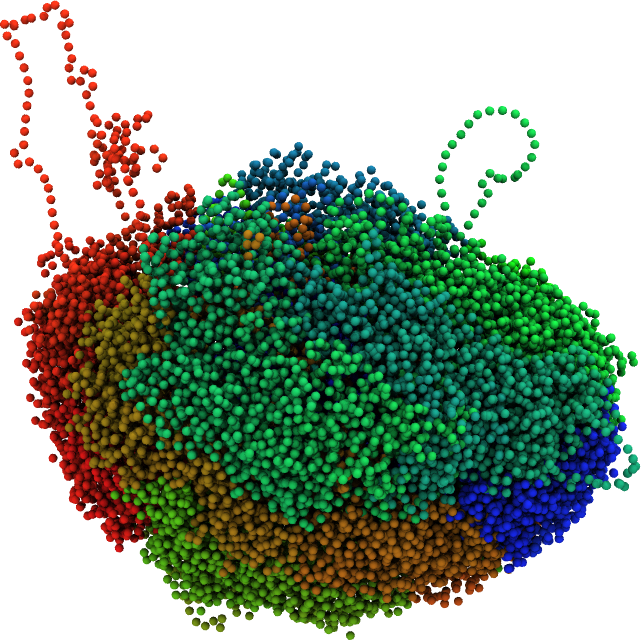
\includegraphics[height=\cellrenderingheight]{cell1_frame104_scene1.png}
  \caption{Cell 1, frame 104, scene 1}
  \label{img:cell1_frame104_scene1}
\end{figure}

\begin{figure}[H]
\centering
  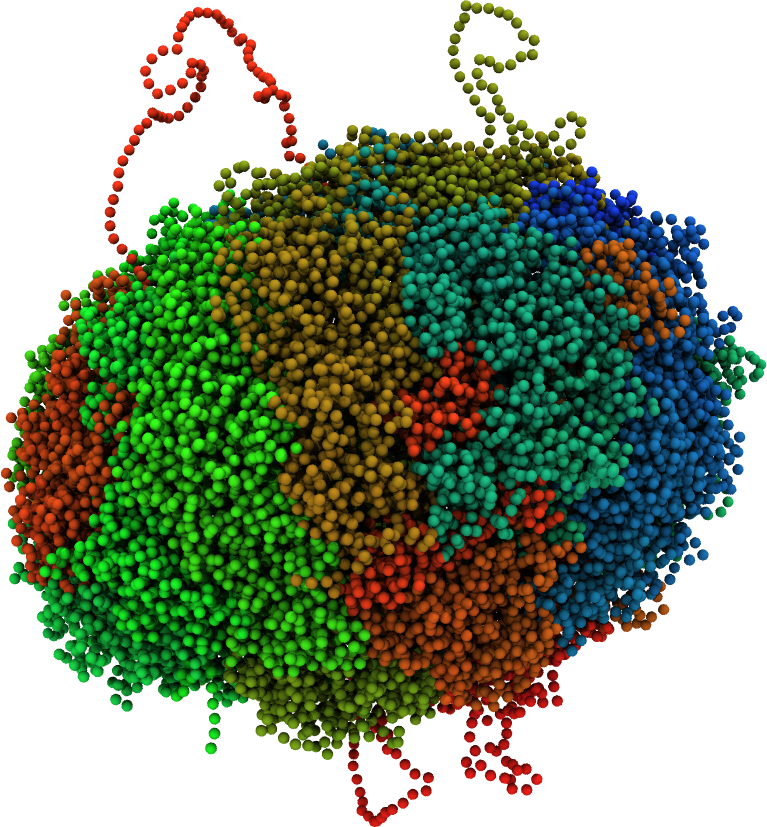
\includegraphics[height=\cellrenderingheight]{cell2_frame104_scene1.png}
  \caption{Cell 2, frame 104, scene 1}
  \label{img:cell2_frame104_scene1}
\end{figure}

\begin{figure}[H]
\centering
  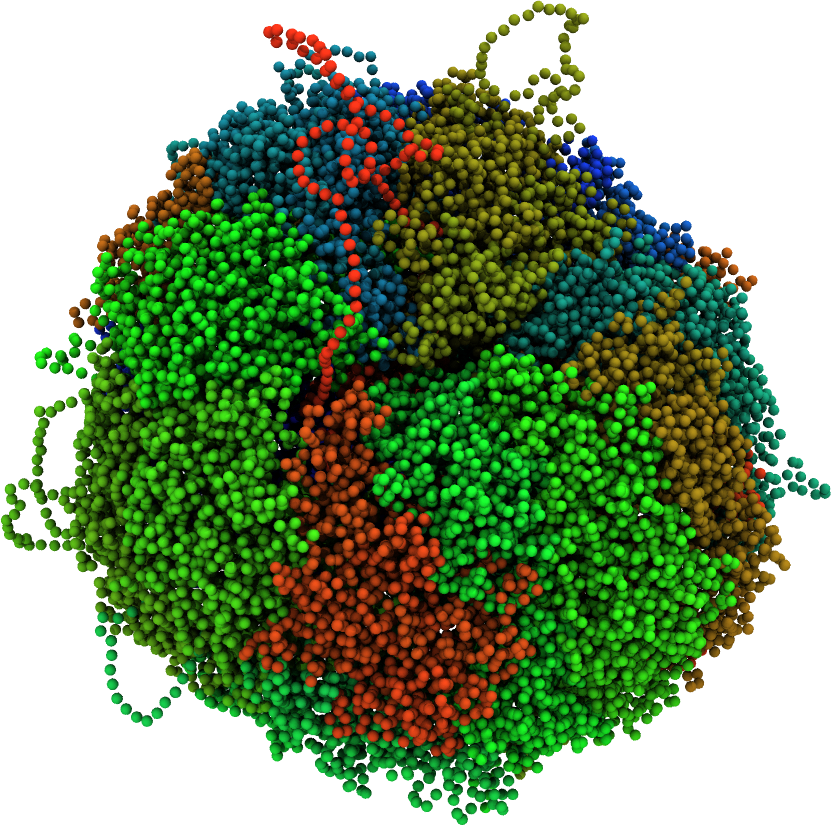
\includegraphics[height=\cellrenderingheight]{cell2_frame104_scene2.png}
  \caption{Cell 2, frame 104, scene 2}
  \label{img:cell2_frame104_scene2}
\end{figure}

\begin{figure}[H]
\centering
  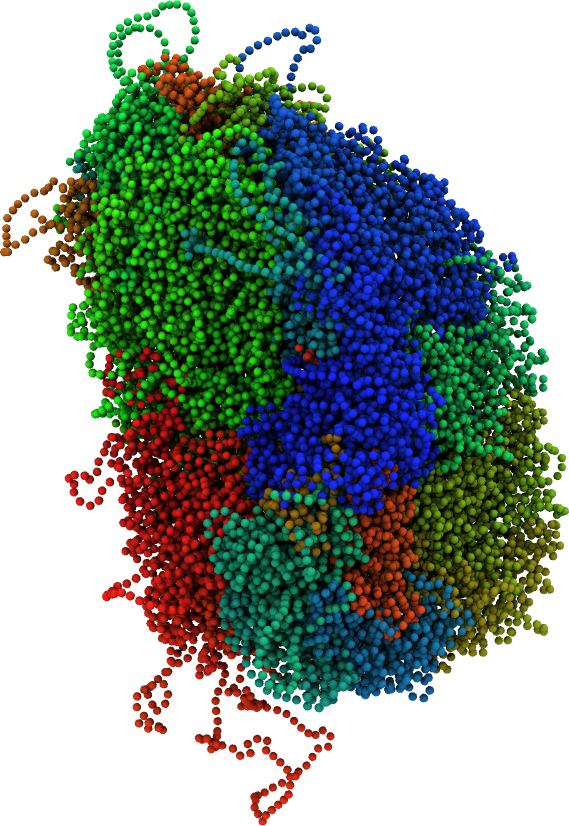
\includegraphics[height=\cellrenderingheight]{cell3_frame104_scene1.png}
  \caption{Cell 3, frame 104, scene 1}
  \label{img:cell3_frame104_scene1}
\end{figure}

\begin{figure}[H]
\centering
  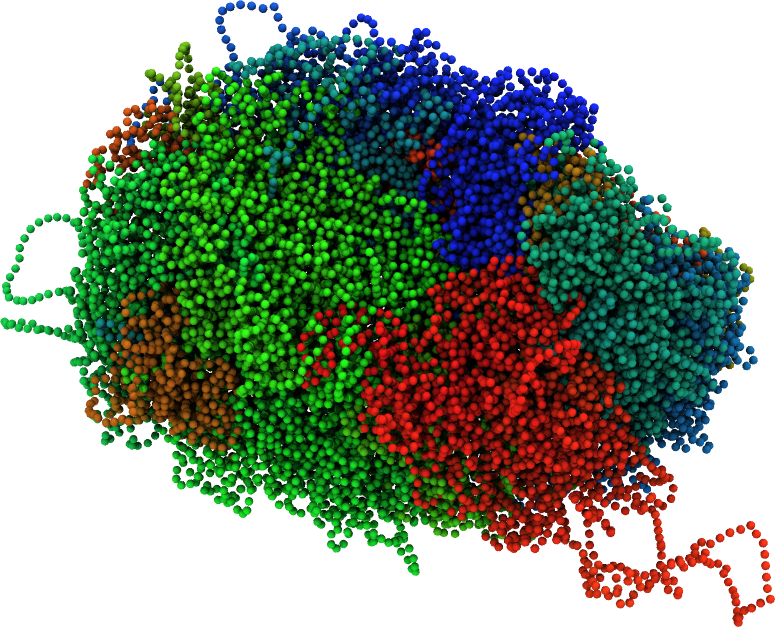
\includegraphics[height=\cellrenderingheight]{cell3_frame104_scene4.png}
  \caption{Cell 3, frame 104, scene 4}
  \label{img:cell3_frame104_scene4}
\end{figure}

\begin{figure}[H]
\centering
  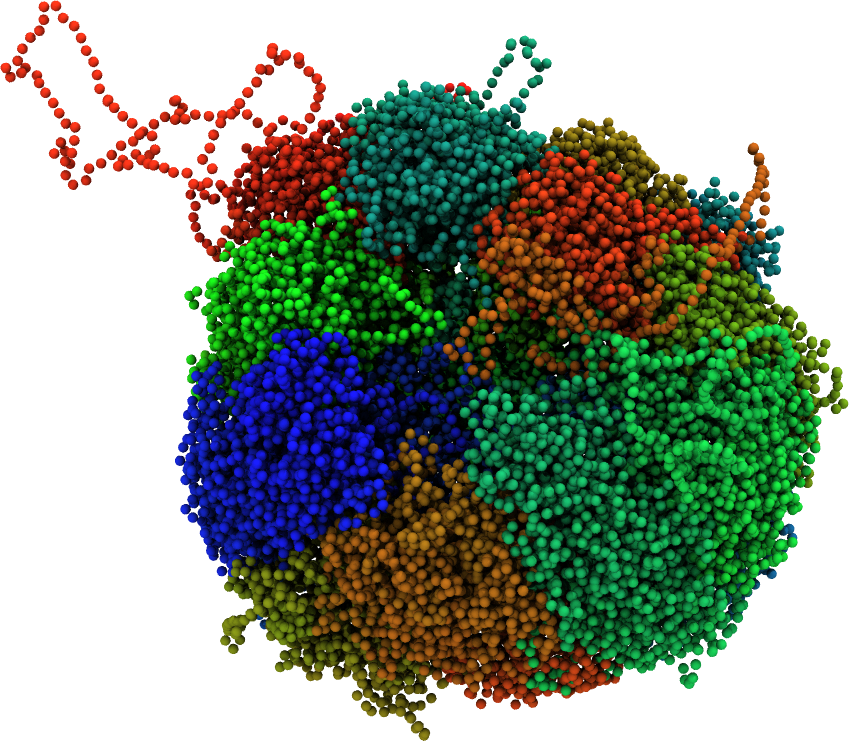
\includegraphics[height=\cellrenderingheight]{cell4_frame104_scene1.png}
  \caption{Cell 4, frame 104, scene 1}
  \label{img:cell4_frame104_scene1}
\end{figure}

\begin{figure}[H]
\centering
  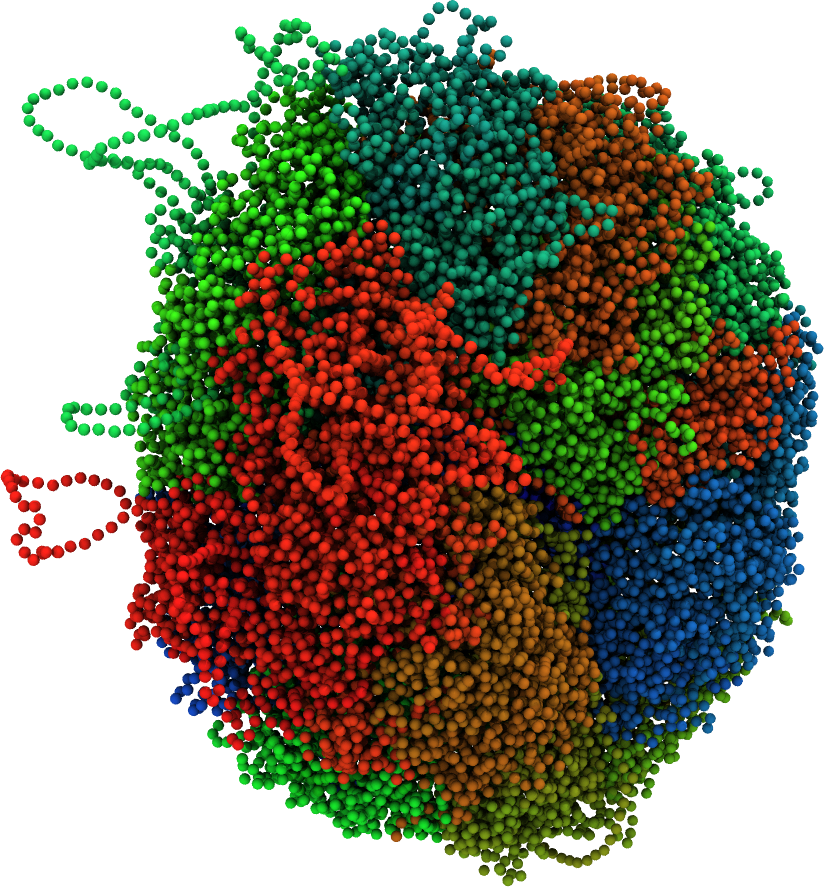
\includegraphics[height=\cellrenderingheight]{cell5_frame036_scene1.png}
  \caption{Cell 5, frame 36, scene 1}
  \label{img:cell5_frame036_scene1}
\end{figure}

\begin{figure}[H]
\centering
  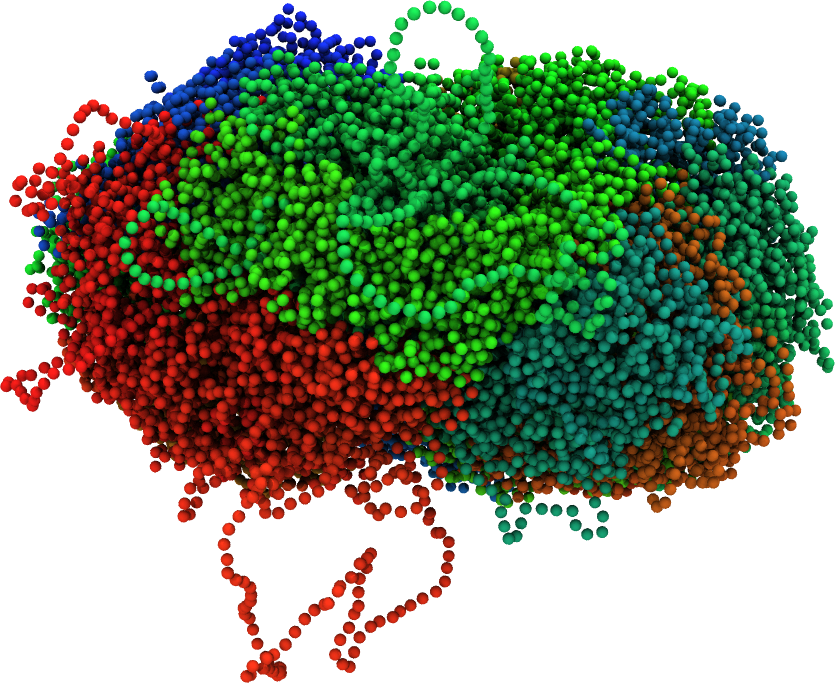
\includegraphics[height=\cellrenderingheight]{cell5_frame036_scene2.png}
  \caption{Cell 5, frame 36, scene 2}
  \label{img:cell5_frame036_scene2}
\end{figure}

\begin{figure}[H]
\centering
  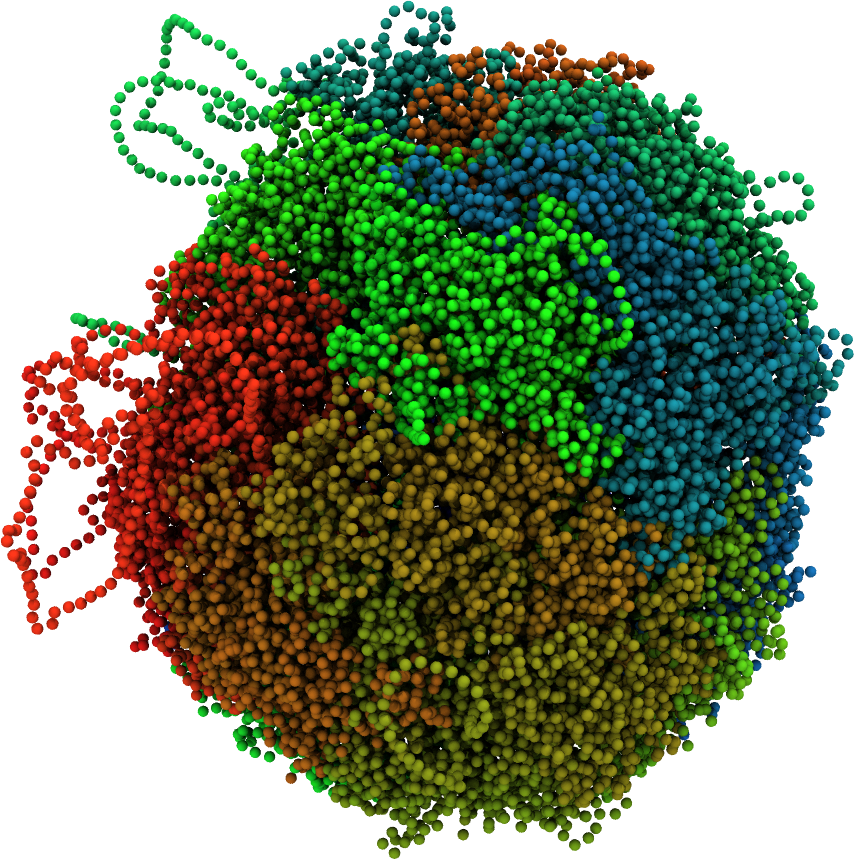
\includegraphics[height=\cellrenderingheight]{cell5_frame104_scene1.png}
  \caption{Cell 5, frame 104, scene 1}
  \label{img:cell5_frame104_scene1}
\end{figure}

\begin{figure}[H]
\centering
  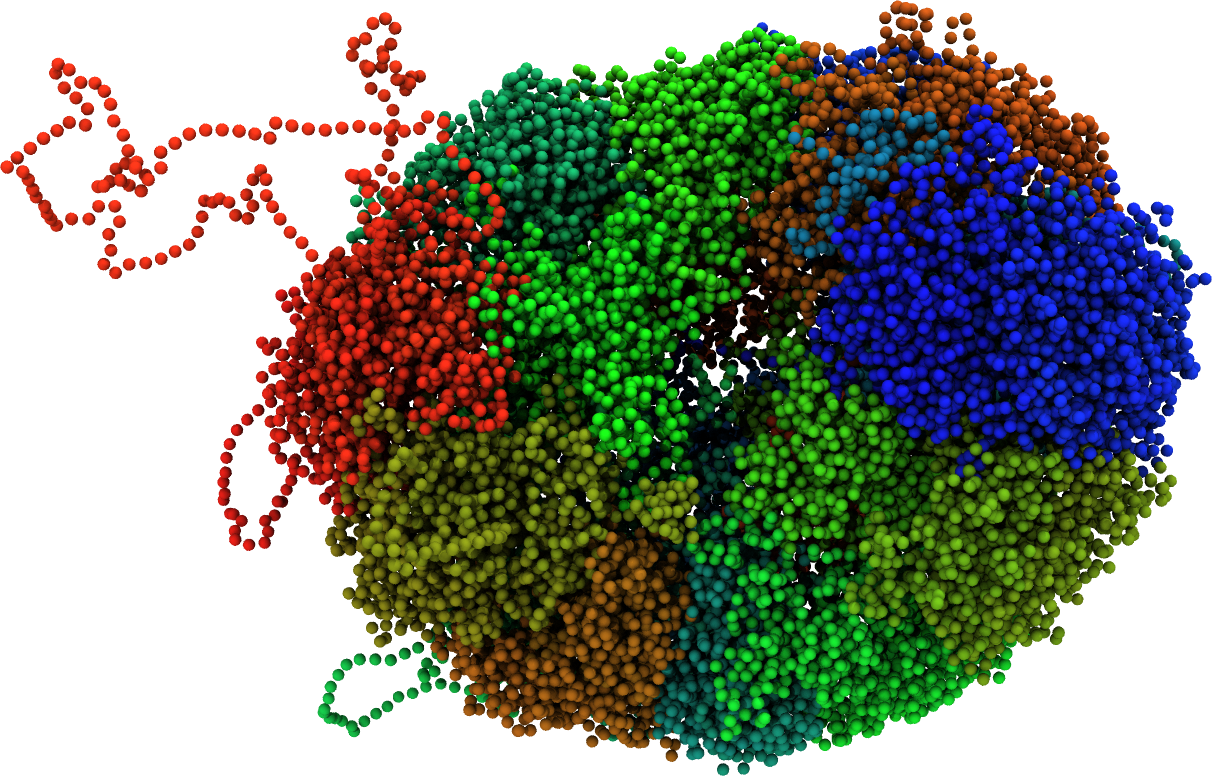
\includegraphics[height=\cellrenderingheight]{cell6_frame104_scene1.png}
  \caption{Cell 6, frame 104, scene 1}
  \label{img:cell6_frame104_scene1}
\end{figure}

\begin{figure}[H]
\centering
  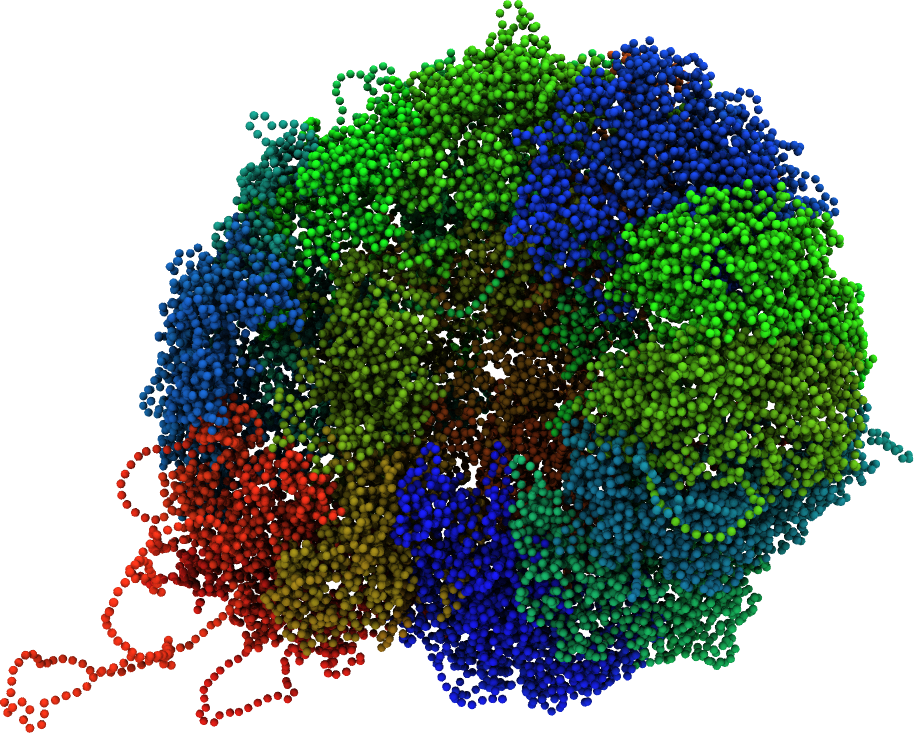
\includegraphics[height=\cellrenderingheight]{cell7_frame104_scene1.png}
  \caption{Cell 7, frame 104, scene 1}
  \label{img:cell7_frame104_scene1}
\end{figure}

\begin{figure}[H]
\centering
  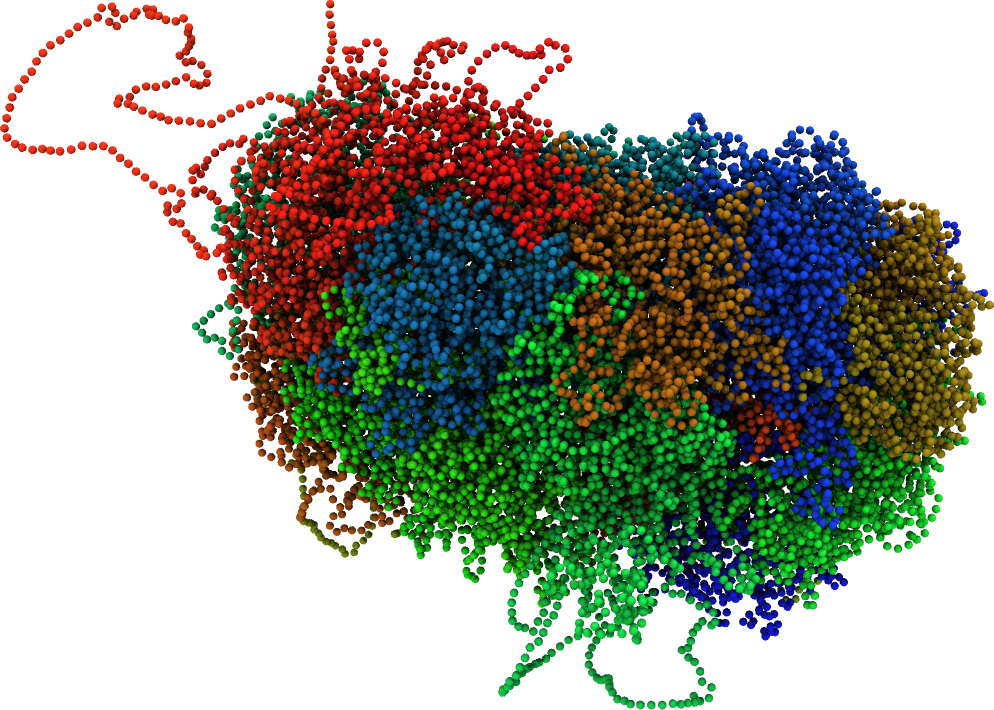
\includegraphics[height=\cellrenderingheight]{cell8_frame104_scene2.png}
  \caption{Cell 8, frame 104, scene 2}
  \label{img:cell8_frame104_scene2}
\end{figure}
